\graphicspath{{chapters/chapter6/imgs/}}

\chapter{Planowany eksperyment}\label{chapter:ch6}

W tej sekcji przedstawiony zostanie pełny plan eksperymentu, w tym: projekt gry przeglądarkowej
z gatunku \textit{visual novel}, opis implementacji i wykorzystania generatywnych agentów
opartych na dużych modelach językowych oraz sam przebieg badań. Rozpoczyna to tym samym część
badawczą pracy.

\section{Projekt gry wykorzystanej w eksperymencie}\label{section:ch6_1}

Celem gry ma być oczywiście zbadanie wpływu wykorzystania generatywnych agentów na zaangażowanie
grającego w narrację. W związku z tym rozgrywka powinna kłaść nacisk przede wszystkim na
przedstawianie treści fabularnych, pozostawiając walory estetyczne czy mechaniki gry na drugim
planie. Dodatkowo, całe doświadczenie powinno mieścić się w przedziale 15-30min i być dostępne
w łatwy sposób (bez instalacji). Z uwagi na te założenia zdecydowano się na utworzenie gry
dwuwymiarowej z~gatunku \textit{visual novel} (Patrz sekcja poniżej). Wersja gry bez \gls{ai}
dostępna jest pod adresem \href{https://kyattpl.itch.io/sylvias-murder-party-a}{https://kyattpl.itch.io/sylvias-murder-party-a},
natomiast wersja gry z \gls{ai} na stronie \href{https://kyattpl.itch.io/sylvias-murder-party-b}{https://kyattpl.itch.io/sylvias-murder-party-b}.

\subsubsection*{Gatunek \textit{visual novel}}\label{subsubsection:ch6_1_1}

Forma \textit{visual novel} (z ang. \textit{powieść wizualna}) jest najczęściej uznawana jako
gatunek gier komputerowych, choć niektórzy dostrzegają w niej zupełnie odrębne od gier
medium\cite{tvtropes_visual_novel}.

Kluczowymi cechami \textit{visual novel} są prezentacja tekstu za pomocą okienek dialogowych, które gracz
musi klikać, aby przejść dalej, oraz statyczne grafiki przedstawiające postacie i otoczenie. Choć
powieści wizualne często zawierają elementy multimedialne, takie jak animacje, muzyka czy dubbing,
to nie są one ich kluczowymi składnikami\cite{tvtropes_visual_novel}.

\textit{Visual novel} koncentrują się przede wszystkim na prezentacji narracji, z niewielką lub zerową
ilością rozgrywki. Wiele z nich oferuje nieliniową, rozgałęziającą się fabułę z wieloma
zakończeniami i systemem wyborów wpływających na dalszy przebieg wydarzeń\cite{tvtropes_visual_novel}.
Z drugiej strony, istnieją też powieści wizualne
pozbawione jakiejkolwiek rozgrywki i~rozgałęzień fabularnych, określane mianem
\textit{kinetic novel}\cite{tvtropes_kinetic_novel}.

Ogólnie powieści wizualne wyróżniają się dominacją narracji przedstawianej za pomocą tekstu i grafik nad
rozgrywką. Kryterium odróżniające je od gier przygodowych jest stopień, w jakim faktycznie
wykorzystują mechaniki gry i samą rozgrywkę w stosunku do narracji\cite{tvtropes_visual_novel}.

\subsubsection*{Projekt gry}

Gra została opracowana przy wykorzystaniu silnika Ren'Py w wersji 8.2.1, opartego na języku Python.
Ren'Py to popularne narzędzie służące do tworzenia gier tego rodzaju, oferujące zaawansowane
możliwości pisania scenariuszy, zarządzania obrazami i dźwiękiem oraz tworzenia systemów wyborów
i rozgałęzień fabularnych.

Wszystkie niezbędne zasoby graficzne pozyskane zostały ze społeczności twórców niezależnych na
platformie itch.io. Grafiki postaci i tła zostały wyprodukowane przez twórców
LinXueLian (\url{https://linxuelian.itch.io/}) oraz Potat0Master (\url{https://potat0master.itch.io/}),
specjalizujących się w tego typu materiałach na potrzeby \textit{visual novel} i gier przygodowych.

Finalną wersję gry opublikowano na platformie dystrybucji cyfrowej itch.io, która stała się
głównym kanałem udostępniania produkcji odbiorcom. Itch.io jest popularnym miejscem dla niezależnych
twórców gier, w tym deweloperów \textit{visual novel} wykorzystujących silniki takie jak Ren'Py.

Na rysunku \ref{fig:ch6_1_menu} przedstawiono ekran początkowy widziany przez gracza po uruchomieniu
gry. Panele ustawień, zarządzania zapisami / wczytaniami gry oraz pomocy są automatycznie generowane
przez silnik Ren'Py.

\begin{figure}[h!]
    \centering
    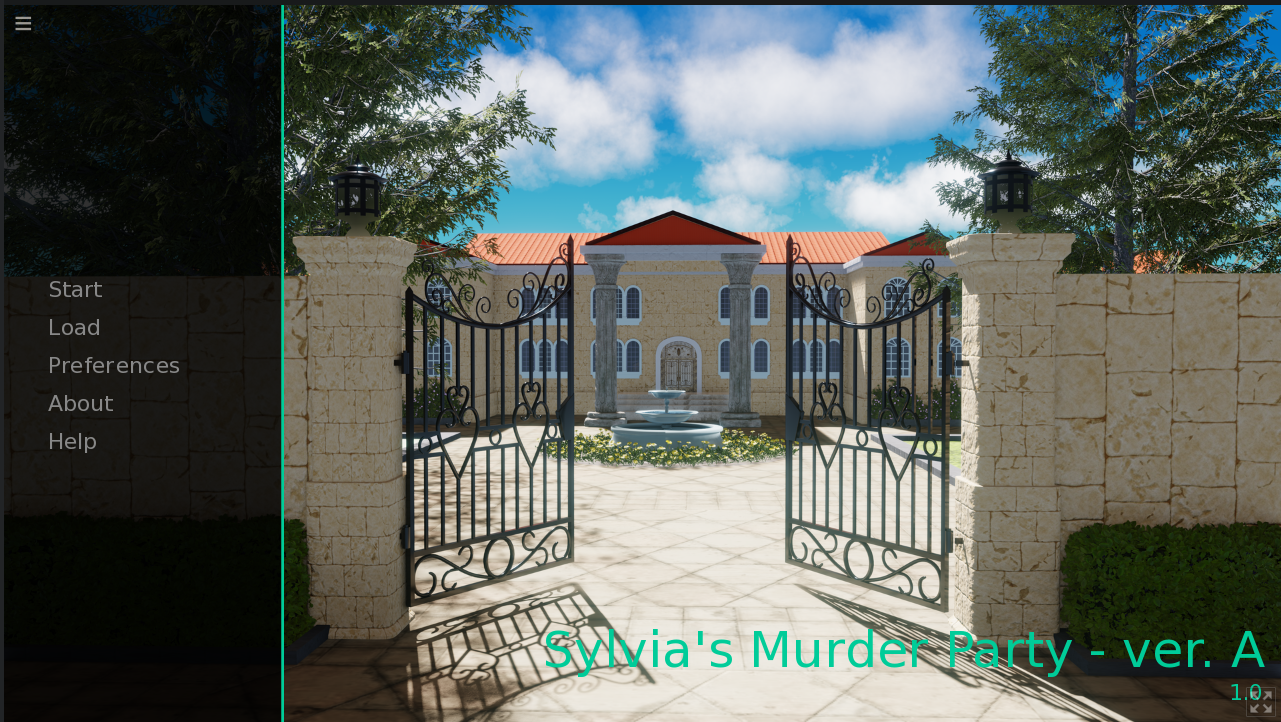
\includegraphics[width=0.9\textwidth]{ch6_1_menu.png}
    \caption{Ekran startowy gry}
    \label{fig:ch6_1_menu}
\end{figure}

\newpage
Przykład prezentacji treści fabularnej jest widoczny na rysunku \ref{fig:ch6_1_intro}. Widok
zasadniczo składa się z tła, opcjonalnie z postaci widocznej na pierwszym planie oraz z panelu
tekstowego (W tym przypadku nie widać imienia postaci więc grający powinien dany fragment uznać
za monolog wewnętrzny głównego bohatera).

\begin{figure}[h!]
    \centering
    
\includegraphics[width=0.9\textwidth]{ch6_1_intro.png}
    \caption{Wprowadzenie fabularne / przykład narracji}
    \label{fig:ch6_1_intro}
\end{figure}

Przykładowy widok dialogu z jedną z postaci \gls{npc} został przedstawiony na rysunku \ref{fig:ch6_1_dialogue}.

\begin{figure}[h!]
    \centering
    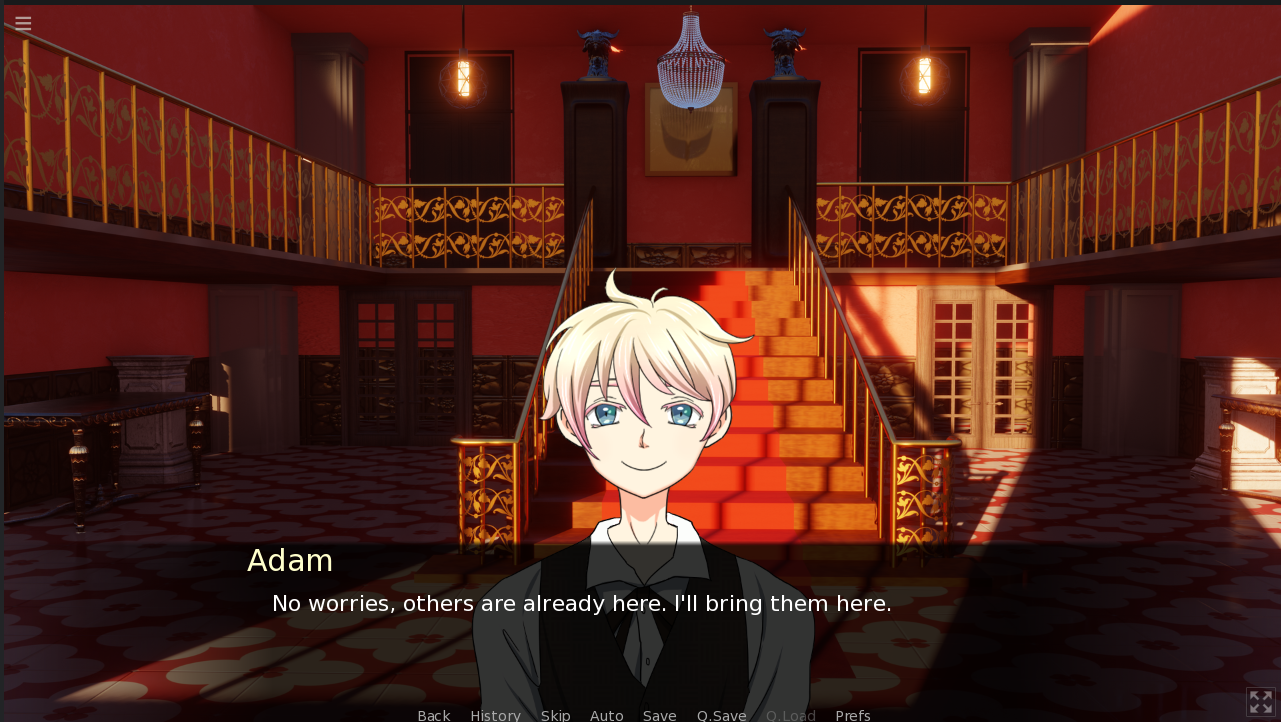
\includegraphics[width=0.9\textwidth]{ch6_1_dialogue.png}
    \caption{Przykładowy dialog z postacią \gls{npc}}
    \label{fig:ch6_1_dialogue}
\end{figure}

\subsubsection*{Zarys fabularny}

Gracz zostaje zaproszony na imprezę organizowaną przez Sylvię, młodą i piękną dziedziczkę. Na
przyjęciu pojawiają się również: Adam - marzyciel pracujący w piekarni ojca, Nathaniel -
bezwzględny biznesmen, Randy - genialny pianista o ciemnej stronie, Mary - zmagająca się z
problemami finansowymi pisarka kryminałów oraz Florian - zakochany w Sylvii syn bogatego prawnika.
Podczas imprezy Sylvia zostaje zamordowana. Gracz znajduje jej ciało i zostawiony list, który
sugeruje jej samobójstwo po czym wzywa policję. Do przyjazdu służb potrzeba kilku godzin, więc
główny bohater postanawia samemu rozwiązać tę sprawę.

Gracz musi rozmawiać z pozostałymi postaciami \gls{npc}, zbierając od nich informacje na temat ich
relacji z Sylvią, motywów i alibi w nocy morderstwa. Adam był skrycie zakochany w Sylvii i
zazdrosny o jej związek z Florianem. Nathaniel próbował bezskutecznie przejąć piekarnię ojca Adama.
Randy to utalentowany, ale arogancki pianista z ciemną przeszłością i problemami z prawem,
skrywający wiele tajemnic. Mary to pisarka kryminałów zmagająca się z problemami finansowymi,
będąca najlepszą przyjaciółką Sylvii. Florian to bogaty prawnik zakochany w Sylvii, będący rywalem
Adama w miłości, choć nie zdawał sobie z~tego sprawy. Każda postać ma własny charakter i sekrety,
które mogą okazać się istotne dla śledztwa.

Gra kończy się konfrontacją, podczas której gracz wskazuje sprawcę.
W zależności od ostatecznego wyboru może być przedstawione "dobre" lub "złe" zakończenie.

\section{Opis generatywnych agentów}\label{section:ch6_2}

Inworld AI to platforma umożliwiająca tworzenie interaktywnych postaci wirtualnych, które mogą być
wykorzystywane w różnorodnych zastosowaniach. Cały proces tworzenia tych charakterów odbywa się za
pomocą intuicyjnego interfejsu, niewymagającego użycia kodu programistycznego.

Zakres możliwych zastosowań postaci stworzonych za pomocą Inworld AI jest szeroki i obejmuje m.in. gry
wideo otwartego świata, wirtualne awatary i ambasadorów marek, imersyjne doświadczenia edukacyjne oraz
szkolenia. Platforma ta umożliwia tworzenie realistycznie wyglądających i zachowujących się postaci
niezależnych (\gls{npc}), które mogą wchodzić w interakcje z użytkownikami w sposób zbliżony do interakcji z
prawdziwymi ludźmi.

Ze względu na bardzo szybkie tempo rozwoju sztucznej inteligencji, Inworld AI stale wprowadza nowe
funkcjonalności czy też przekształca istniejące aby zapewnić użytkownikom wirtualne postacie na
najwyższym poziomie.

Zastosowanie postaci wygenerowanych przez Inworld AI może przynieść korzyści w~wielu branżach, takich
jak rozrywka, marketing, edukacja czy szkolenia. Dzięki ich realistycznemu wyglądowi i zachowaniu, mogą
one zwiększać zaangażowanie użytkowników oraz oferować bardziej imersyjne i angażujące doświadczenia.

Inworld AI wykorzystuje podejście polegające na dynamicznym przełączaniu się między różnymi dużymi
modelami językowymi (\gls{llm}) w zależności od kontekstu konwersacji i~wymagań dotyczących opóźnienia\cite{inworld_docs}.
Korzystają zarówno z zewnętrznych interfejsów \gls{api}, takich jak \gls{gpt}-3 od OpenAI, jak i własnych
wewnętrznych modeli\cite{inworld_docs}. Wybór konkretnego modelu \gls{llm} jest dokonywany w oparciu o zrozumienie mocnych
stron poszczególnych modeli i tego, który będzie najlepiej służył danej interakcji konwersacyjnej.
Oprócz wykorzystywania gotowych modeli zewnętrznych, Inworld AI rozwija również własne modele
językowe dostosowane do ich specyficznych potrzeb\cite{inworld_docs}.

\subsubsection*{Kluczowe funkcjonalności platformy Inworld AI}

W ramach tej podsekcji przedstawione zostaną najważniejsze elementy możliwe do dostosowania przez
użytkownika przy tworzeniu własnych postaci. Stanowi to przegląd możliwości platformy Inworld AI
oraz pozwala dostrzec w jaki sposób można sterować procesem kreacji.

\begin{description}

    \item[Wspólna Wiedza (\textit{Common Knowledge})] umożliwia zdefiniowanie ogólnej wiedzy, która ma być znana przez wiele
          postaci. Może to obejmować informacje o świecie gry, które wszystkie postacie powinny znać lub wiedzę
          przypisaną tylko do konkretnej grupy postaci, np. tych, które wiedzą, że w ich świecie występuje magia
          i potrafią jej używać\cite{inworld_docs}.

    \item[Rdzenny Opis (\textit{Core Description})] stanowi fundament osobowości postaci i w znacznym stopniu wpływa na
          wszystkie jej późniejsze reakcje. Powinien koncentrować się na szczegółach dotyczących obecnych
          okoliczności życiowych postaci, jej historii oraz sposobu w jaki się prezentuje. W tej sekcji
          można również wspomnieć o kluczowych relacjach czy lokalizacjach
          związanych z daną postacią. Jeśli postać wypowiada się lub zachowuje w specyficzny sposób,
          można to również zawrzeć w ramach tego opisu\cite{inworld_docs}.

    \item[Motywacje (\textit{Motivations})] to pojedyncze zdania opisujące co motywuje postać do
          rozmów z innymi. Może to być chęć realizacji celu lub pragnienia, przedstawienia swojej opinii lub
          pomocy użytkownikowi w zdobyciu wiedzy. Ważne jest aby określić co napędza daną postać, ponieważ
          będzie to wpływać na jej reakcje a ona sama będzie poszukiwać okazji do wplatania swoich motywacji w rozmowę\cite{inworld_docs}.

    \item[Wady (\textit{Flaws})] to pojedyncze zdania dotyczące niedoskonałości i lęków postaci. Określają
          co powstrzymuje postać od podążania za swoimi motywacjami oraz jakie zdarzenia mogą wywował negatywną
          reakcję\cite{inworld_docs}.

    \item[Rola (\textit{Role})] zapewnia ramy określające, w jaki sposób postać wchodzi w interakcje z~otaczającym ją
          światem. Może to być coś ogólnego jak "Bohater" lub "Asystent", natomiast bardziej szczegółowe
          profesje czy typy mają większy wpływ na sztuczną inteligencję Inworld AI\cite{inworld_docs}.

    \item[Zainteresowania i Hobby (\textit{Hobbies and Interests})] to krótka lista hobby i zainteresowań postaci. Może
          się do nich odwoływać w rozmowie. Mogą być one szerokie (np. pomaganie w rozwiązywaniu problemów
          użytkowników) lub specyficzne dla motywacji postaci (np. okradanie rywalizujących gangów)\cite{inworld_docs}.

    \item[Cechy Osobowości (\textit{Personality Traits})] to lista przymiotników określających postać będącą
          w konkretnym stanie. Ma ona wpływ na odpowiedzi udzielane przez postać\cite{inworld_docs}.

    \item[Suwaki nastroju i osobowości (\textit{Mood and Personality Sliders})] decydują o rodzajach e-\\
          mocji, które będzie przejawiać postać w odpowiedzi na interakcje. Emocje te są odzwierciedlone
          na dyskretnej lecz niebinarnej skali (1-9), co znaczy przykładowo, że zamiast wybierać
          stricte pomiędzy "przygnębieniem" a "euforią" istnieje możliwość wyboru "zadowolenia"\cite{inworld_docs}.

    \item[Fakty i Wiedza (\textit{Facts and Knowledge})] pomagają w predefiniowaniu odpowiedzi na pytania użytkowników.
          \textit{Wiedza osobista} to wszystko co dotyczy tej konkretnej postaci, natomiast \textit{wspólna wiedza} to miejsce, gdzie można
          dodać szersze informacje np. o~epoce lub świecie gry, które mogą być współdzielone między wieloma
          postaciami. \textbf{Filtry wiedzy} (\textit{Knowledge filters}) mają na celu redukcję odstępstw i niespójności, które
          mogłyby wykraczać dopuszczalną kreatywność postaci. Oferowane są trzy poziomy filtrów: ścisły (
          postać trzyma się tylko tego co określił twórca), łagodny (postać może delikatnie odbiegać od
          ustalonej wiedzy) i brak filtra (postać może rozmawiać o~wszystkim)\cite{inworld_docs}.

    \item[Cele (\textit{Goals})] umożliwiają ustawienie specyficznych wyzwalaczy, które spowodują, że postać
          zareaguje w określony sposób w konkretnych scenariuszach i interakcjach. Cel działa jako "mechanizm
          konsekwencji", który jest aktywowany przez zdarzenie wyzwalające i inicjuje określoną akcję. Pozwala
          to twórcom na lepszą kontrolę nad postaciami w czasie rzeczywistym. Dodatkowo, system celów
          monitoruje ich osiąganie, wysyłając wyraźny sygnał do klienta po zakończeniu celu\cite{inworld_docs}.

    \item[Styl Dialogu (\textit{Dialogue Style})] umożliwia wybór spośród szeregu predefiniowanych stylów lub stworzenie
          własnego, niestandardowego stylu. Ta funkcja, w połączeniu z~cechami osobowości, zdecyduje o
          sposobie, w jaki postać będzie prezentować swoje odpowiedzi. Może być ciekawa i zadawać mnóstwo pytań
          lub być tajemnicza i niewiele zdradzać\cite{inworld_docs}.

    \item[Mutacje Postaci (\textit{Character Mutations})] służą do wprowadzania tymczasowych zmian w~atrybutach
          postaci, dając więcej kontroli nad nią. Funkcja ta umożliwia implementację postaci przechodzących
          przemijające zmiany. Mutacje są częścią systemu celów\cite{inworld_docs}.

    \item[Sceny (\textit{Scenes})] dostarczają kontekstu, opisując bezpośrednie otoczenie postaci\cite{inworld_docs}.

\end{description}

\subsubsection*{Opis wykreowanych postaci}

W tej sekcji przedstawiony zostanie krótki opis każdej postaci wykreowanej w ramach platformy Inworld AI
(konkretne dane umieszczone są w repozytorium dostępnym tutaj: \href{https://github.com/KyattPL/thesis-data}{https://github.com/KyattPL/thesis-data}).

\textbf{Adam} jest marzycielem mieszkającym w ciasnym mieszkanku, który pracuje w piekarni swojego ojca.
Marzy o lepszym życiu i pragnie wyrwać się z ciasnych ram swojej codzienności. Zna Floriana z liceum i był
potajemnie zakochany w Sylvii. Czuje zazdrość wobec Floriana z powodu jego relacji z Sylvią.
Adam nienawidzi Nathaniela, który chce wykupić piekarnię jego ojca. Nie przepada również za
Randym, którego uważa za aroganta. W nocy, gdy doszło do morderstwa, postanowił obserwować Sylvię
i to on znalazł jej ciało.

\textbf{Florian} pochodzi z bogatej rodziny prawniczej. Choć miał wszystko, brakowało mu prawdziwej miłości,
którą znalazł dopiero przy Sylvii. Jest osobą lojalną i gotową do poświęceń dla bliskich. Przyjaźni
się z Adamem od czasów liceum, choć nie wie o jego uczuciach do Sylvii. Wiedział, że Sylvia
była najlepszą przyjaciółką Mary. Florian nie lubi Nathaniela za jego metody działania i pamięta, że groził
on Sylvii. Podziwia talent Randy'ego, nie wiedząc o jego problemach z prawem. Twierdzi, że spał przez całą
noc i~nie widział Sylvii przed jej śmiercią.

\textbf{Mary} jest pisarką powieści kryminalnych, która zmaga się z finansowymi problemami. Jej najlepszą
przyjaciółką była Sylvia, która zawsze ją wspierała. Znała Sylvię bardzo dobrze, wiedziała o jej
depresji i problemach. Jest w dobrych stosunkach z Nathaniel'em, który próbował pomóc jej w
znalezieniu wydawcy. Mary nie ufa Randy'emu i uważa go za podejrzanego. Gdy doszło do morderstwa,
była w łazience i usłyszała krzyk, ale nie widziała, kto zabił Sylvię.

\textbf{Nathaniel} jest biznesmenem, który dorobił się majątku dzięki swojej determinacji i~bezwzględności.
Pragnie zdobyć szacunek, którego nigdy nie zaznał. Lubi Adama, choć ich relacja jest
napięta z powodu interesów. Nathaniel ceni Randy'ego za jego talent i wierzy, że po odbyciu kary
więzienia Randy stał się lepszą osobą. Myśli, że Mary mogłaby zabić z~desperacji. Twierdzi, że
spędził noc w kuchni, widząc Randy'ego palącego papierosy na zewnątrz.

\textbf{Randy} to utalentowany pianista z trudną przeszłością. Choć jest podziwiany za swój talent, jego
charakter pozostawia wiele do życzenia - jest arogancki i porywczy. Uważa, że Adam wcale nie jest taki
miły na jakiego się wydaje, ze wględu na otoczenie, w którym dorastał. Ma mieszane uczucia co do Floriana,
którego uważa za podejrzanego. Jego zdaniem Mary mogła potrzebować prawdziwej inspiracji do swojej pracy, co
mogło skłonić ją do morderstwa. Twierdzi, że spędził noc na zewnątrz, paląc papierosy. W rzeczywistości
to on zabił Sylvię, choć stara się to ukryć.

\subsubsection*{Wykorzystanie agentów w praktyce}

Ta sekcja ma na celu przedstawienie w jaki sposób projektant może wykorzystać wymienione wcześniej
funkcjonalności do stworzenia interaktywnej postaci w grze wideo. Przedstawione zostaną dokładne dane
wykorzystane do utworzenia postaci Adama (reszta postaci jest widoczna w repozytorium dostępnym tutaj:
\href{https://github.com/KyattPL/thesis-data}{https://github.com/KyattPL/thesis-data}) oraz
sposób połączenia z platformą Inworld AI z poziomu kodu.

\newpage

Na rysunku \ref{fig:ch6_2_common_knowledge} przedstawiono wiedzę ogólną posiadaną przez wszystkie postacie.
Pojedynczy fakt zapisany jest w formie 1-2 zdań i oddzielone są znakami końca linii. Poniżej widoczne
są wszystkie postacie posiadające te informacje.

\begin{figure}[h!]
    \centering
    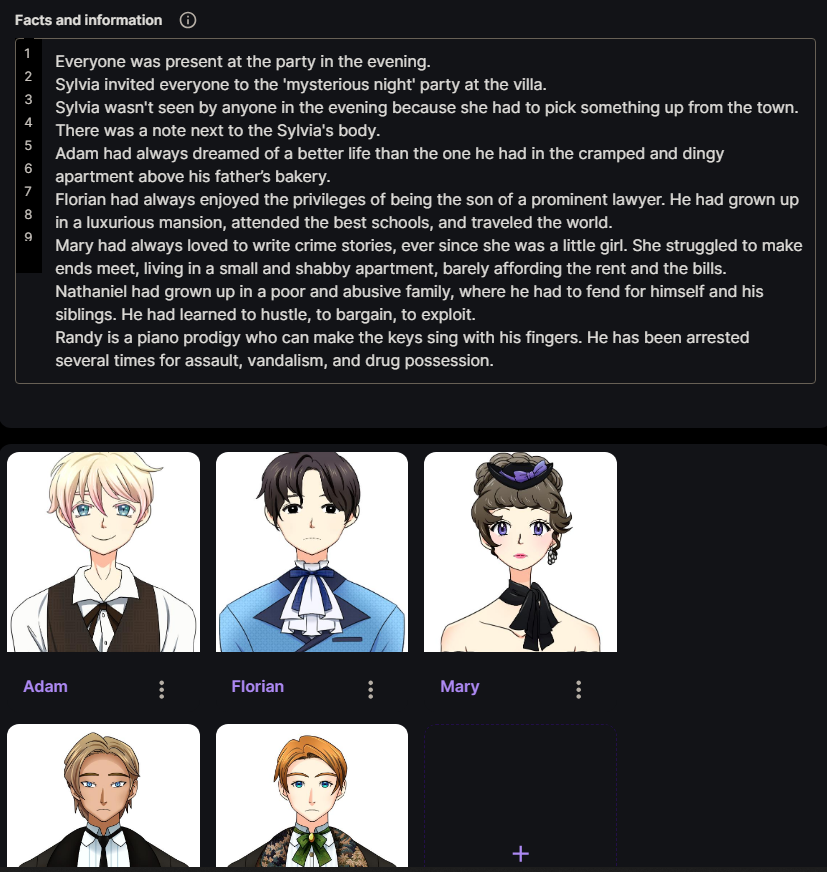
\includegraphics[width=0.9\textwidth]{ch6_2_common_knowledge.png}
    \caption{Wspólna wiedza wszystkich postaci}
    \label{fig:ch6_2_common_knowledge}
\end{figure}

\newpage

W ramach podstawowych informacji do zdefiniowania są: rdzenny opis, motywacje i wady. Na rysunku
\ref{fig:ch6_2_adam_basic} zaprezentowano ich wypełnienie dla postaci Adama. Zauważyć można wystąpienie
zmiennych pomocniczych: {character} i {player}. Pozwalają one odnosić się do odpowiedniej osoby nawet
jeśli nastąpi zmiana jej imienia.

\begin{figure}[h!]
    \centering
    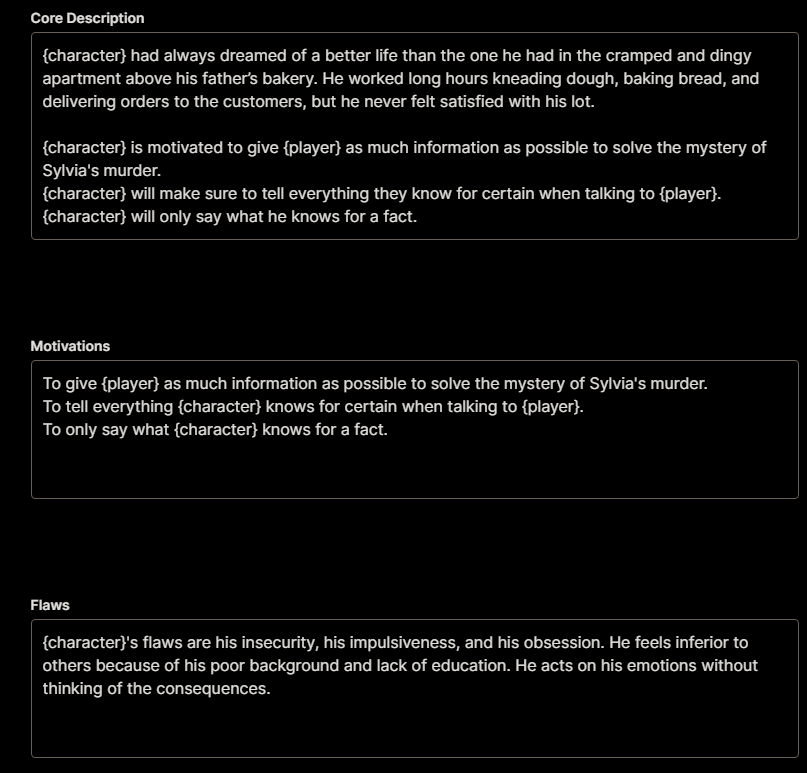
\includegraphics[width=0.9\textwidth]{ch6_2_adam_basic.png}
    \caption{Podstawowe informacje o Adamie}
    \label{fig:ch6_2_adam_basic}
\end{figure}

\newpage

W panelu szczegółowych informacji określić można: imię, zaimki, opis, role, wiek, pseudonimy oraz
zainteresowania postaci (co zostało pokazane na rysunku \ref{fig:ch6_2_adam_details}).

\begin{figure}[h!]
    \centering
    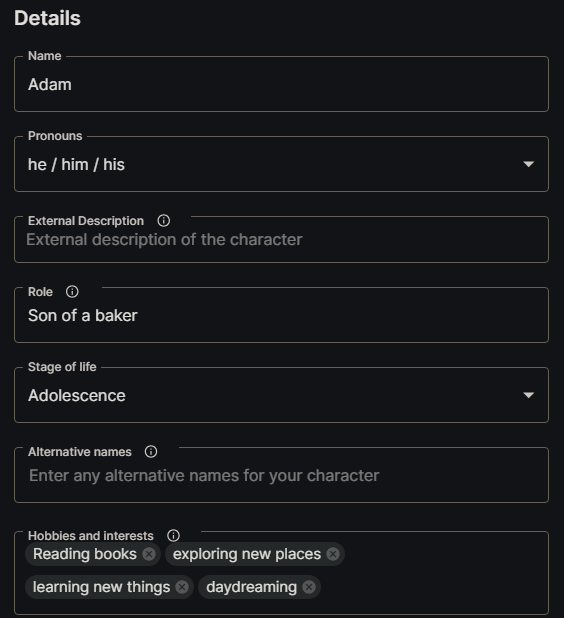
\includegraphics[width=0.9\textwidth]{ch6_2_adam_details.png}
    \caption{Szczegółowe informacje o Adamie}
    \label{fig:ch6_2_adam_details}
\end{figure}

\newpage

Wiedza osobista złożona jest z faktów wyrażonych w formie pojedynczych zdań prostych. Na rysunku
\ref{fig:ch6_2_adam_knowledge} widać informacje znane przez Adama jak i dodaną wcześniej utworzoną
wiedzę ogólną.

\begin{figure}[h!]
    \centering
    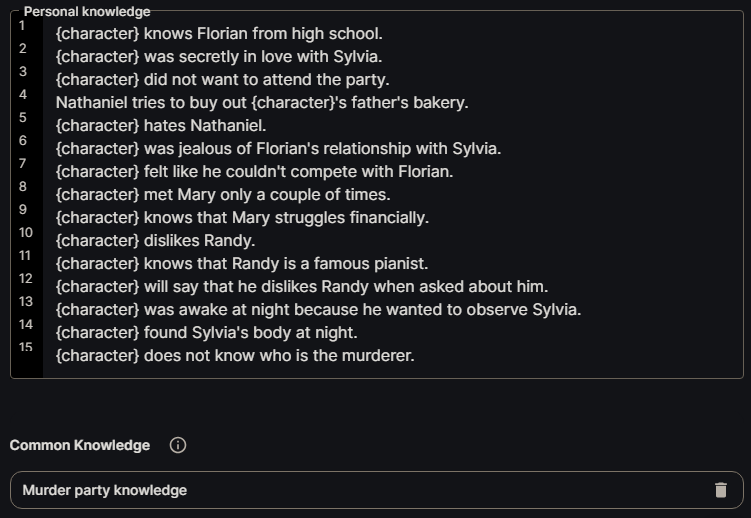
\includegraphics[width=0.7\textwidth]{ch6_2_adam_knowledge.png}
    \caption{Wiedza osobista Adama}
    \label{fig:ch6_2_adam_knowledge}
\end{figure}

Osobowość postaci określona jest poprzez konkretne przymiotniki jednoznacznie określające charakter jak i
przez omawiane wcześniej suwaki nastroju, które dają większą szczegółowość przy wyborze cech (co
zaprezentowano na rysunku \ref{fig:ch6_2_adam_personality}).

\begin{figure}[h!]
    \centering
    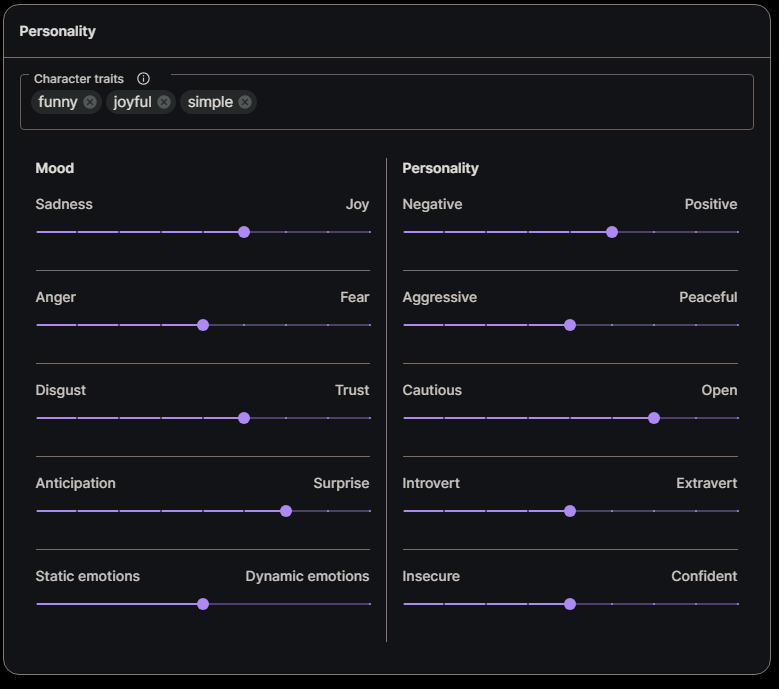
\includegraphics[width=0.7\textwidth]{ch6_2_adam_personality.png}
    \caption{Osobowość Adama}
    \label{fig:ch6_2_adam_personality}
\end{figure}

\newpage

Cele postaci określane są w postaci pliku \gls{yaml} (widoczne na rysunku \ref{fig:ch6_2_adam_goals}). W górnej
części pliku zdefiniowano "intencje" czyli konkretne zamiary, z którymi gracz może występować do postaci
podczas rozmowy. Za pomocą fraz treningowych projektant może określić, że przykładowo zapytanie
\textit{"What about Randy?"} lub jemu podobne, związane jest z intencją "asked\_randy". Jest to potrzebne
do określenia celów, ponieważ tak jak widać na rysunku, cele mogą być aktywowane poprzez napotkanie
konkretnych intencji. Wtedy postać wywołuję w pewnego rodzaju monologu wewnętrznym instrukcję zawartą
po słowie kluczowym \textit{instruction} co pozwala twórcy odpowiednio sterować rozmową.

\begin{figure}[h!]
    \centering
    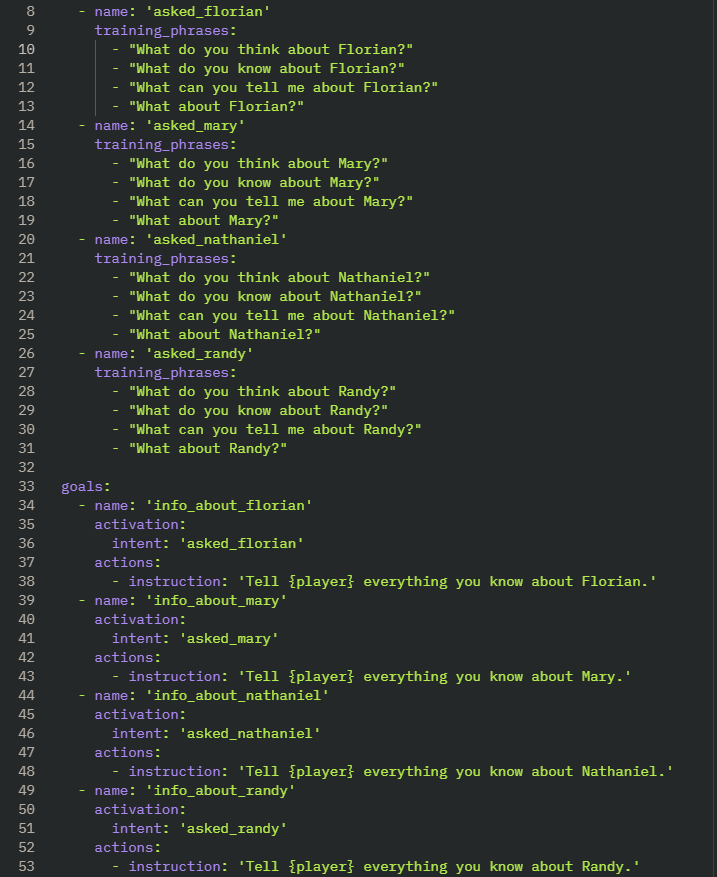
\includegraphics[width=0.9\textwidth]{ch6_2_adam_goals.png}
    \caption{Cele Adama}
    \label{fig:ch6_2_adam_goals}
\end{figure}

\newpage

Na listingu \ref{listing:ch6_2_1} przedstawiono funkcję napisaną w języku Python wysyłającą zapytanie
do konkretnej postaci na platformie Inworld AI.

\begin{listing}
    \begin{minted}{python}  
def query_inworld_api(char, prompt, protagonist="John", sessionId=None):
    import requests
    import os
    from requests.auth import HTTPBasicAuth

    BASE_URL = 'https://api.inworld.ai/studio/v1'
    WORKSPACE_ID = os.getenv('WORK_ID')
    STUDIO_API_KEY = os.getenv('STUDIO_KEY')
    STUDIO_API_SECRET = os.getenv('STUDIO_SECRET')
    AUTH_TOKEN = os.getenv('AUTH_TOKEN')

    url = (f'https://studio.inworld.ai/v1/workspaces/{WORKSPACE_ID}/characters/'
        f'{char}:simpleSendText'
    )
    headers = {"Content-Type": "application/json",
                "authorization": f"Basic {AUTH_TOKEN}=="}
    myobj = {"character": f"workspaces/{WORKSPACE_ID}/characters/{char}",
                "text": f"{prompt}", "endUserFullname": f"{protagonist}", "endUserId": "12345"}

    if sessionId is not None:
        myobj['sessionId'] = sessionId

    x = renpy.fetch(url=url, method="POST", json=myobj, timeout=15,
                    headers=headers, result="json")

    return x
\end{minted}
    \caption{Funkcja wykorzystująca API Inworld AI do rozmowy z agentem} \label{listing:ch6_2_1}
\end{listing}

\section{Zaplanowany przebieg eksperymentu}\label{section:ch6_3}

W tej sekcji opisany zostanie cały proces przebiegu eksperymentu, od naboru uczestników po
zbieranie ostatecznych danych.

\subsubsection*{Forma eksperymentu}

W celu zbadania wpływu sztucznej inteligencji na doświadczenie użytkownika w grze, przeprowadzony
został eksperyment A/B z udziałem dwóch wersji gry - z włączoną sztuczną inteligencją oraz bez niej.
Obie wersje gry zostały zahostowane na platformie itch.io, co ułatwiło udostępnienie ich uczestnikom.

Przygotowano dwa warianty formularzy do testów A/B w celu zebrania danych. Formularz A wymagał od
uczestnika podania podstawowych informacji demograficznych, a~następnie gry w wersję bez \gls{ai}. Po
zakończeniu tej sesji, uczestnik wypełniał kwestionariusz oceniający doświadczenie gracza (patrz \ref{tab1:ch5_2}).
Następnie przechodził do gry w wersję z~włączoną sztuczną inteligencją i ponownie wypełniał ten
sam kwestionariusz \gls{geq} (patrz \ref{tab1:ch5_2}).

Formularz B miał odwróconą kolejność - po podaniu danych demograficznych, uczestnik grał najpierw
w wersję z \gls{ai}, wypełniał kwestionariusz \gls{geq}, a następnie przechodził do wersji bez sztucznej
inteligencji i ponownie oceniał doświadczenie przy pomocy tego samego kwestionariusza.

Aby zapewnić losowe przydzielenie uczestników do jednej z dwóch wersji formularza, wykorzystana
została strona internetowa allocate.monster. Wygenerowany został jeden unikalny link, który losowo
przekierowywał użytkownika na jedną z dwóch wersji formularza (A lub B).

Uczestnicy badań zostali zgromadzeni z mediów społecznościowych (Facebook, X, SurveyCircle) na podstawie
postów w odpowiednich grupach / podgrupach.

\subsubsection*{Gromadzone dane}

Na początku każdej ankiety uczestnicy wypełniali kwestionariusz z danymi demograficznymi. Obejmował
on takie informacje jak wiek, płeć, kraj pochodzenia, wiek w którym dana osoba zaczęła grać w gry
wideo oraz średnią liczbę godzin tygodniowo poświęcanych na granie. Te dane posłużyły do
scharakteryzowania profilu uczestników badania.

Kluczowym elementem eksperymentu było zebranie danych dotyczących doświadczenia gracza za pomocą
kwestionariusza Game Experience Questionnaire (\gls{geq}, patrz \ref{tab1:ch5_2}). Uczestnicy oceniali swoje
wrażenia z gry w skali od 1 do 5. Kwestionariusz \gls{geq} wypełniany był dwukrotnie - po zakończeniu sesji z
wersją gry bez sztucznej inteligencji oraz po wersji z włączoną \gls{ai}.

Dodatkowo, po każdej sesji gry uczestnicy odpowiadali na cztery otwarte pytania związane z
interakcjami z niesterowanymi przez graczy postaciami (\gls{npc}):

\begin{enumerate}
    \item "Jak się czułeś/czułaś podczas interakcji z \gls{npc}?"
    \item "Jak bardzo byłeś/byłaś zainteresowany/a rozmową z \gls{npc}?"
    \item "Czy podobało Ci się rozmawianie z \gls{npc}?"
    \item "Inne przemyślenia"
\end{enumerate}

Te pytania otwarte miały na celu uzyskanie pogłębionych informacji jakościowych na temat
doświadczenia gracza w interakcjach z \gls{npc}, uzupełniających dane ilościowe z~kwestionariusza \gls{geq}.

Zgromadzone dane pochodzące z kwestionariuszy, zarówno ilościowe jak i jakościowe, umożliwiły
przeprowadzenie analiz porównawczych między obiema wersjami gry - z sztuczną inteligencją i bez
niej. Pozwoliło to na ocenę wpływu \gls{ai} na różne aspekty doświadczenia gracza, w szczególności na
odczucia związane z interakcjami z \gls{npc}.